\subsection{Ion Orbit Loss} \label{sub:IOL}

\acf{IOL} represents a non-diffusive mechanism for losing particles. At the heart of \ac{IOL} theory is an electromagnetic equilibrium argument that, to a first order, between any two flux surfaces canonical angular momentum (\cref{eqn:IOLCanonAngleMom}), energy (\cref{eqn:IOLEnergy}), and magnetic moment (\cref{eqn:IOLMagMom}) are conserved. Based on this fundamental principle, \citeauthor{Miyamoto1996} \cite{Miyamoto1996} observed that one could use the values of plasma parameters on an inner flux surface (marked with a subscript 0) and the parameters on a separatrix, (marked with a subscript s or no subscript). \prettyref{fig:featuressofatokamakplasma} illustrates two flux surfaces, one being the separatrix and an inner one between the core and edge region.

\begin{equation}
	\left[ R\, m\, V_\parallel \left(\cfrac{B_\varphi}{B}\right) + e \psi \right]_0
	=
	\left[ R\, m\, V_\parallel \left(\cfrac{B_\varphi}{B}\right) + e \psi \right]_s 
	\label{eqn:IOLCanonAngleMom}
\end{equation}

\begin{equation}
	\left[ \cfrac{1}{2} \left( V_\parallel^2 + V_\perp^2  \phantom{\cfrac{1}{2}}\right) \right]_0
	=
	\left[ \cfrac{1}{2} \left( V_\parallel^2 + V_\perp^2  \phantom{\cfrac{1}{2}}\right) \right]_s
	\label{eqn:IOLEnergy}	
\end{equation}

\begin{equation}
	\left[ \cfrac{m\,V_\perp^2}{2\,B} \right]_0
	=
	\left[ \cfrac{m\,V_\perp^2}{2\,B} \right]_s
	\label{eqn:IOLMagMom}
\end{equation}

Utilizing \cref{eqn:IOLV0}, defining the term $f_\varphi$ in \cref{eqn:IOLfphi} and the parameter $\zeta_0$, which is the direction cosine of the particles launch angle with respect to the toroidal magnetic field line, $B_\varphi$, \crefrange{eqn:IOLCanonAngleMom}{eqn:IOLMagMom} can be rewritten into \cref{eqn:IOLMinV0}. This equation, which is quadratic in $V_0$, represents the equilibrium velocity for a particle to have an orbit that is within the confined portion of the plasma, meaning within the separatrix.

\begin{equation}
	V_0 = \sqrt{V_\parallel^2 + V_\perp^2}
	\label{eqn:IOLV0}
\end{equation}

\begin{equation}
	f_\varphi = \left|\cfrac{B_\varphi}{B}\right|
	\label{eqn:IOLfphi}
\end{equation}

\begin{equation}
	\zeta_0 = \cfrac{V_{\parallel 0}}{V_0}
	\label{eqn:IOLzeta0}
\end{equation}

This then serves as the criterion for which a particle can be lost. If it has an energy in excess of this, then it will have an orbit outside of the confined plasma and can encounter a variety of obstructions, such as magnetic field imperfections, \ac{SOL} particles, and most obviously, the wall. The manner by which this minimum velocity is applied to calculate a loss estimate is described in \cref{subsub:CumulativeLoss}.

\begin{equation}
	\begin{gathered}
			V^2_0 \left[ \left( \cfrac{R_0}{R} \cfrac{f_{\varphi 0}}{f_{\varphi}} \zeta_0 \right)^2 -1 + 
		\left( 1 - \zeta^2_0 \right) \left| \cfrac{B}{B_0} \right|  \right] + 
		V_0 \left[ \cfrac{2e \left( \psi_0 - \psi \right) }{R m f_\varphi} \left( \cfrac{R_0}{R}  \cfrac{f_{\varphi 0}}{f_\varphi} \zeta_0 \right)^{\vphantom{2}}   \right] \\
		+ \left[ \left( \cfrac{e\left( \psi_0 - \psi \right) }{R m f_\varphi} \right)^2 - \cfrac{2 e \left(\phi_0 - \phi  \right) }{m} \right] = 0
	\end{gathered}
	\label{eqn:IOLMinV0}
\end{equation}

\prettyref{fig:iolCalc} shows the minimum energy calculations against plasma ion temperature, what this illustrates is that \ac{IOL} is not a dominant transport mechanism for the plasma core. However, it becomes the dominant effect in the last 5\% \cite{Stacey2013} and drives the features in this region.

\begin{figure}
	\centering
	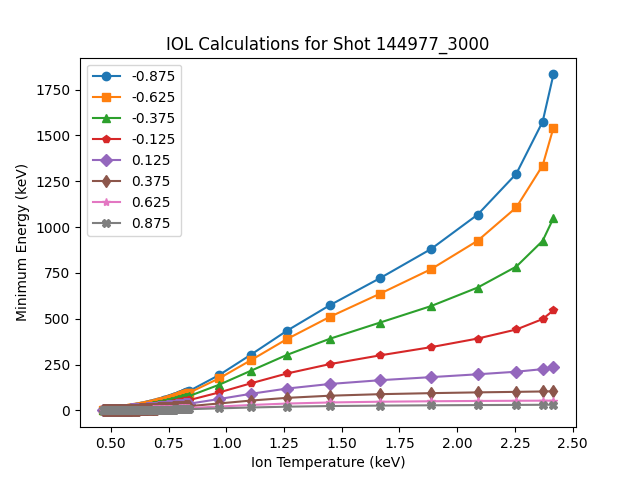
\includegraphics[width=0.5\linewidth]{images/iol_calculations}
	\caption[IOL Calculation]{Minimum Energy calculation for Shot 144977.3000}
	\label{fig:iolCalc}
\end{figure}


\subsubsection{Cumulative Loss Fraction} \label{subsub:CumulativeLoss}

The temperature of any flux surface is assumed to be Maxwellian in the velocity space, which means that if one assumes a three dimensional velocity space, the distribution of energy is given by a Gamma distribution as illustrated in \prettyref{fig:maxwellianGeneral}. The cumulative loss fraction, $F_{rj}^{IOL}$, is determined by truncating the distribution above the minimum energy given in \cref{eqn:IOLEmin}. This leads to an evaluation of the incomplete Gamma distribution, $\BbbGamma$, at $\epsilon\left(\rho,\zeta_0\right)$. The zeroth moment, which corresponds to particle loss, results in a $\BbbGamma\left(\frac{3}{2}\right)$ shown in \cref{eqn:IOLCumulativeLossParticle}. The first moment, which corresponds to momentum loss, results in $\BbbGamma\left(2\right)$ shown in \cref{eqn:IOLCumulativeLossMomentum}. The second moment, which corresponds to energy loss, results in $\BbbGamma\left(\frac{5}{2}\right)$ shown in \cref{eqn:IOLCumulativeLossEnergy}.

\begin{equation}
	\epsilon_{min} = \cfrac{1}{2} m \, V_0^2
	\label{eqn:IOLEmin}
\end{equation}

\begin{figure}[!hb]
	\subfloat[Core Region] {
		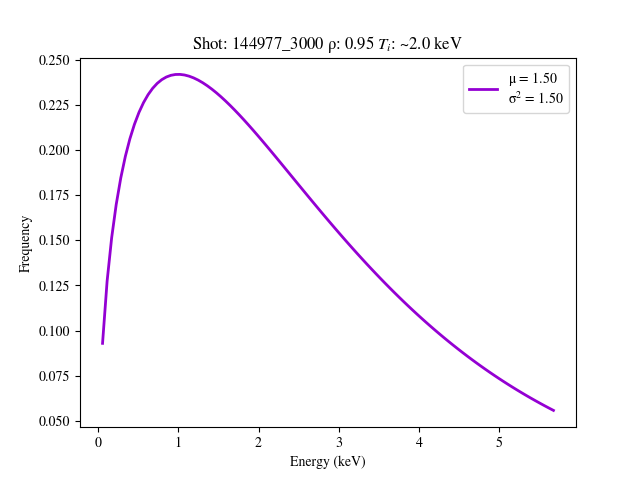
\includegraphics[width=0.5\linewidth]{images/maxwellian_illustration}
		\label{fig:maxwellianGeneral}
	} \quad
	\subfloat[$\rho=0.98$, $T_i=0.517 keV$] {
		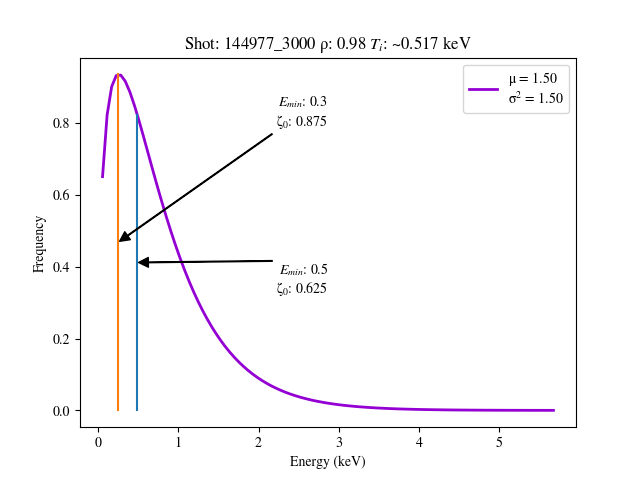
\includegraphics[width=0.5\linewidth]{images/maxwellian_illustration_144977_3000_rho976}
		\label{fig:maxwellianEdge}
	}
	\caption{Maxwellian Gamma Distribution for shot 144977.3000}
\end{figure}

One aspect of the \ac{IOL} that is important to note is that the equilibrium given by \crefrange{eqn:IOLCanonAngleMom}{eqn:IOLMagMom} identify which particles have energy that take them beyond the \ac{LCFS}, but this does not necessarily imply loss. Instead it implies a sufficient orbit to enter unfavorable zones. From this observation, one has to postulate that a certain number of these particles will either i) suffer a collision in the \ac{SOL}, which is not collisionless and therefore reasonable, or ii) particles strike the wall. With this in mind, we utilize the Stacey rational approximation that $R_{loss}^{IOL}$ is approximately 0.5, the logic being that some is more likely than none, while all is probably too much. Half is about right.

\begin{equation}
	F_{rj}^{IOL} \left( r \right) = \cfrac{N_{loss}}{N_{total}} = \cfrac{R_{loss}^{IOL} \bigints_{-1}^{1} \left[ \bigintss_{V_{0,min}}^{\infty} V_0^2 f\left( V_0 \right) dV_0\right] d \zeta_0}{2 \bigintss_{0}^{\infty} V_0^2 f\left(V_0\right)dV_0} = 
	\cfrac{R_{loss}^{IOL} \bigints_{-1}^{1} \BbbGamma \left(\cfrac{3}{2}, \epsilon_{min}\left(\rho,\zeta_0\right)   \right) d\zeta_0}{2 \BbbGamma \left(\cfrac{3}{2}\right)}
	\label{eqn:IOLCumulativeLossParticle}
\end{equation}

\begin{equation}
	M_{rj}^{IOL} \left( r \right) = \cfrac{M_{loss}}{M_{total}} = 
	\cfrac{R_{loss}^{IOL} \bigints_{-1}^{1} \left[ \bigintss_{V_{0,min}}^{\infty} 
		\left(m\,V_0\,\zeta_0\right) V_0^2 f\left( V_0 \right) dV_0\right] d\zeta_0}{2 \bigintss_{0}^{\infty} \left(m\,V_0\right) V_0^2 f\left(V_0\right)dV_0} = 
	\cfrac{R_{loss}^{IOL} \bigints_{-1}^{1} \BbbGamma \left(2, \epsilon_{min}\left(\rho,\zeta_0\right)   \right) d\zeta_0}{2 \BbbGamma \left(2\right)}
	\label{eqn:IOLCumulativeLossMomentum}
\end{equation}


\begin{equation}
	E_{rj}^{IOL} \left( r \right) = \cfrac{E_{loss}}{E_{total}} = \cfrac{R_{loss}^{IOL} \bigints_{-1}^{1} \left[ \bigintss_{V_{0,min}}^{\infty} \left(\cfrac{1}{2} m\,V_0^2\right) V_0^2 f\left( V_0 \right) dV_0\right] d\zeta_0}{2 \bigintss_{0}^{\infty} \left(\cfrac{1}{2} m\,V_0^2\,\zeta_0\right) V_0^2 f\left(V_0\right)dV_0} = 
	\cfrac{R_{loss}^{IOL} \bigints_{-1}^{1} \BbbGamma \left(\cfrac{5}{2}, \epsilon_{min}\left(\rho,\zeta_0\right)   \right) d\zeta_0}{2 \BbbGamma \left(\cfrac{5}{2}\right)} 
	\label{eqn:IOLCumulativeLossEnergy}
\end{equation}

